\section{Tuesday, March 21st: Data Analysis}
\subsection{Managing Study Participants}
It can be a stressful experience for Participants, which is why we follow the 3 Belmont Principles.

What kind of questions are you asking about -- is it a sensitive topic that they don't feel comfortable sharing?

Are you going to give literal personally-identifiable info? Or will you deal in \textit{aggregates} (as you should).

\begin{shaded}
Ask yourself the question: Will the person be identifiable from the information shared?
\end{shaded}

\subsection{Treating Subjects with Respect}
If you are doing this at a University, you need to go through IRB (Institutional Review Board).

How to let people in the study know:
\begin{itemize}
    \item Give them a consent form which they must read and sign -- you don't need to make this from scratch -- most universities have tools to generate such a form with correct legal dictation.
    \item Keep a copy of the form, while making sure the participant has a copy
\end{itemize}

Don't waste their time -- debug your experiments beforehand \& have everything ready.

Make users comfortable (this is a big thing in VR studies where wearing the headsets for extended periods of time can become tiresome).

\subsection{Data Analysis}
Now that you have the data, how do you analyze?

\subsubsection{Bubble Cursor Attributes}
\paragraph{Hypotheses}
\begin{itemize}
    \item Quicker
    \item More accurate/Less Errors
\end{itemize}
\myparagraph{Independent Variable}
Cursor type (bubble vs normal).\\
Placement of the bubbles ($D$ in Fitts' Law).\\
Size ($S$ in Fitts' Law).

\paragraph{Dependent Variable}
\begin{enumerate}
    \item Time
    \item Accuracy
\end{enumerate}

\myparagraph{Control Variables}
Think about this yourself!

\myparagraph{Random Variable}
Think about this yourself!

\myparagraph{Control Variables}
Resulting data: usually in a .CSV file.

Attributes:
\begin{itemize}
    \item Unique ID
    \item Cursor Type
    \item Size
    \item How many times it took
    \item Time
    \item etc
\end{itemize}

\subsubsection{Counting Analysis}
We can make descriptive statistics such as:
\[
    \mu = \frac{\sum_{i=1}^N X_i}N
\]
\[
    \sigma = \sqrt\frac{\sum_{i=1}^N (X_i-\mu)^2}N
\]
\myparagraph{Continuous Data}
\textbf{Central tendency}:
\begin{itemize}
    \item mean
    \item median
    \item mode
\end{itemize}
\textbf{Dispersion}:
\begin{itemize}
    \item Range (max-min)
    \item Standard deviation
\end{itemize}
\textbf{Shape of distribution}:
\begin{itemize}
    \item Skew
    \item Kurtosis
\end{itemize}

\myparagraph{Categorical Data}
Frequency Distributions (Note that there is more you can do here (i.e. error bars).

\subsubsection{Cleaning Data}
If you don't visualize your data, you may have no idea that you have a bunch of bad data points -- that need to be removed.

\subsubsection{Skewed Distributions}
The Median is more robust to outliers.
\myparagraph{Negative skew}
$\text{mean} < \text{median} < \text{mode}.$
\myparagraph{Positive skew}
$\textbf{mode} < \textbf{median} < \textbf{mean}$.

\subsubsection{Power Law Distributions}
The distribution of photographers contributing photos of the \textit{2005 Coney Island Mermaid Parade} is carried by a few contributors doing 100+ photos, and the rest doing much less (for an average of 26, and median of 11).
\[p(x) \propto x^{-\alpha}\]

\subsubsection{Confidence Intervals}
95\% Confidence Interval: The range of values in which we’re 95\% sure the true population mean falls.

This can be calculated with the help of the standard error SE.

Standard Deviation: measures variability of individual data points.

Standard Error: measures variability of means
\[\text{SE}=\frac{\text{SD}}{\sqrt{N}}\]
\[
95 \% \text{CI} = \text{M} \pm 1.96 \times \text{SE}
\]

\subsubsection{Hypothesis Testing}
Hypothesis: Manipulation of IV effects DV in some way\\
Null hypothesis: Manipulation of IV has no effect on DV\\\
Null hypothesis assumed true unless statistics allow us to reject it
\myparagraph{p-values}
We need a cutoff for results to be significant 
$p < 0.05$ usually considered significant (Sometimes $p < 0.01$).\\
Means that $< 5$\% chance that null hypothesis is true -- Likelihood that results are due to chance variation.

\subsection{Statistical tests}
\begin{itemize}
    \item T-test (1 factor, 2 levels)
    \item Correlation
\item ANOVA (1 factor, $>2$ levels, multiple factors)
\item MANOVA ($>1$ dependent variable)
\end{itemize}
When to use which test:\\
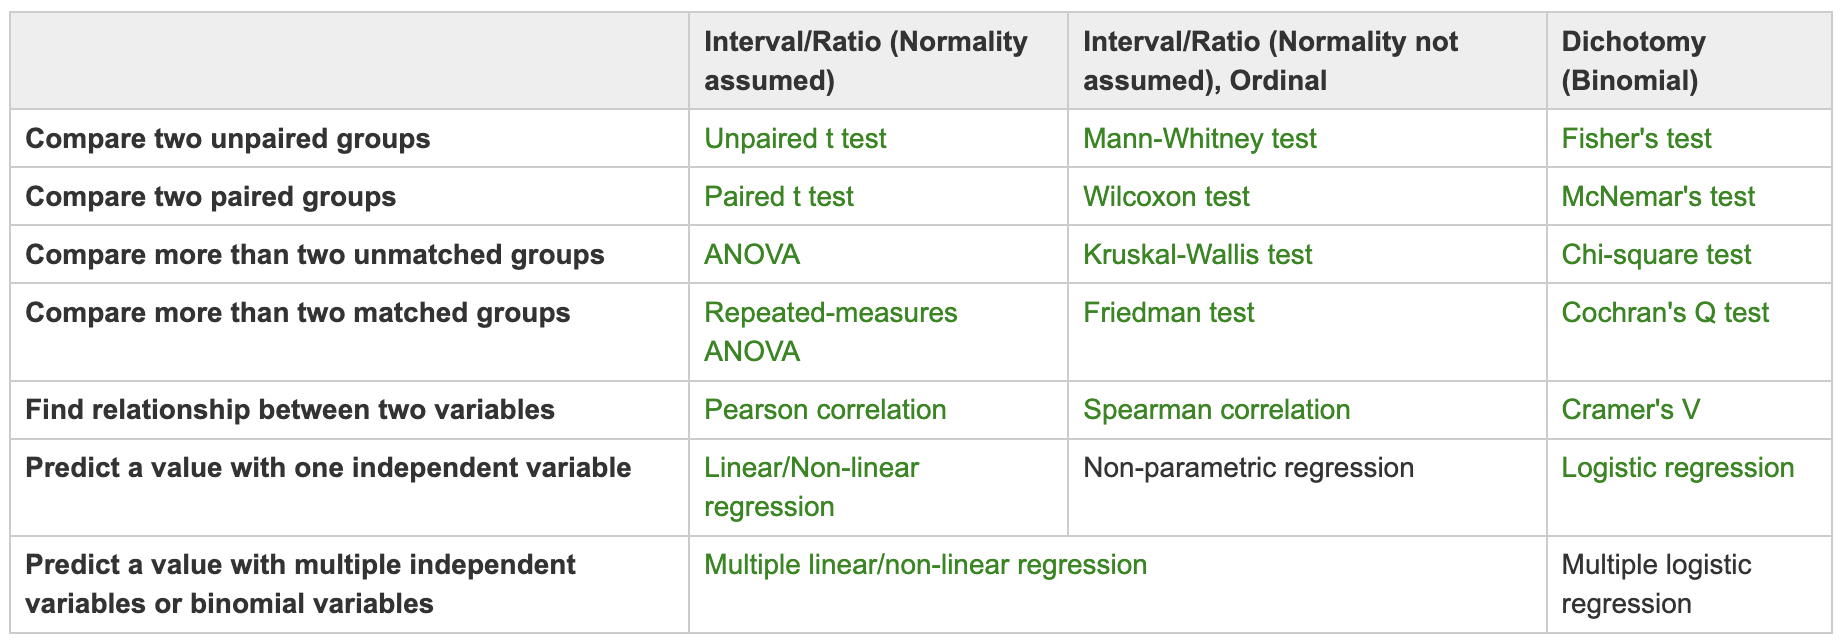
\includegraphics[scale=.25]{lectures/wk10/tests.png}

\subsubsection{Between-subject study: Unpaired vs Paired}
Between-subject study: We cut our participants into 2 groups, which each group trying a different cursors. This is an unpaired group.

If everyone used both cursors, then it matters that these measurements both came from the same person as that would be paired groups.

\subsubsection{t-Test}
1 independent variable with 2 levels,\\
1 dependent variable of type Q (quantitative/interval)

Compares the means of 2 groups\\
Null hypothesis: No difference between means

\myparagraph{Assumptions}
\begin{itemize}
    \item \textbf{Samples are normally distributed}
    \item Very robust in practice
    \item \textbf{Population variances are equal (between subjects tests)}
    \item Reasonably robust for differing variances
    \item \textbf{Individual observations in samples are independent}
\end{itemize}

$t$-Test is somewhat robust to variations in skew as long as the distribution looks somewhat normal.

This is a parametric test.

\subsubsection{Mann-Whitney's U Test}
1 independent variable with 2 levels,\\
1 dependent variable of type O (ordinal), or type Q 
when assumption of normal distribution does not hold.\\
Compares the ranks of values of 2 groups

This is a non-parametric test.

\subsubsection{Parametric vs non-parametric}
t-Tests are parametric as it makes the assumption on the data's distribution (that it is normal). 

Non-parametric test are when one does not rely on a particular distribution.

\myparagraph{When to use non-parametric tests}
Preference data is the most frequently produced ordinal data (Strongly Agree vs Agree vs Neutral vs Disagree vs Strongly Disagree -- so one should use a non-parametric test here).

\subsubsection{ANOVA}
\textbf{Single factor analysis of variance (ANOVA)}:\\
Compare means for 3 or more levels of a single independent variable.

\textbf{Multi-Way Analysis of variance (n-Way ANOVA)}:
Compare more than one independent variable\\
Can find interactions between independent variables

ANOVA tests whether means differ, but does not tell us \textit{which means} differ -- for this we must perform pairwise t-tests.

\subsubsection{Objective measurements}
\begin{itemize}
    \item Good internal validity $\to$ repeatability
    \item \textbf{But, real-world implications may be difficult to foresee\\
Significant results doesn’t imply real-world importance}\\
3.05s versus 3.00s for menu selection
\end{itemize}
